\section{Renormalization Group and Scattering for Scalar Field Theory}
Recall - in PT we have counterterms to cancel out the infinities (because real data shouldn't have infinities). There are a few different renormalization scheme, and this is something that comes up for sure in QFT II where one studies strong interactions, QCD, Non-abelian gauge theories etc. As we've learned there is not really scheme-dependence on the final results, only scheme-dependence of the intermediate steps.

There are still a few things left to clean up from scalar field theory. One is the renormalization group, and the other is scattering theory/S-matrix.

\subsection{Renormalization Group}
We come to this from the least intuitive direction, that being renormalized quantum field theory. The condensed matter theorists have a much better approach to this, where one analyzes a second order phase transition of a classical model. On that side this is much clearer what one is doing. Here, it looks more like a mathematical trick, but unfortunately that's just how it looks from this perspective.

We have a parameter $\mu^2$ that appeared when we were doing renormalization. This was just something we stuck in for dimensional regularization. If we did some kind of other regularization, there would be some other parameter - likely some kind of mass or momentum cutoff which we take to be large. 

In 4-d, the coupling constant is dimensionless. But if we slide below 4 dimensions, it doesn't make sense to say something is large or small because dimensional quantities have to be small in relation to something. So, here we separated out $\mu$ as the dimensional part of the coupling constant to deal with this dimensionality. However, it does not go away when we come back to 4-dimensions, so it is there as another parameter in the theory. In some ways it is a parameter, but we are allowed to take advantage of the fact that it is completely arbitrary.

Let us go back to our theory before we introduced things like counterterms - calculating a correlation function, we have:
\begin{equation}
    Z^{n/2}\Gamma(k_1, \ldots k_n)
\end{equation}
which is just the correlation function in the renormalized theory times the factor $Z^{n/2}$. Note - the mass always stays a mass in any dimension of spacetime, so it is only $\lambda$ that grows a dimensional part in different spacetime dimensions. But looking at the above, nothing depends on $\mu$ at this level. So, we take advantage of this by writing:
\begin{equation}
    \mu \dpd{}{\mu}\left(z^{n/2}\Gamma(k_1 \ldots k_n)\right) = 0
\end{equation}
but this equation is not sensible because $Z$ becomes infinite, so let us introduce an extra factor:
\begin{equation}
    z^{-n/2}\mu\dpd{}{\mu}\left(z^{n/2}\Gamma(k_1 \ldots k_n)\right) = 0
\end{equation}
what happened to the $\mu$-dependence? The bare quantities $m^2 z_m, \lambda \mu^{4-2w}z_\lambda$ do not depend on $\mu$. They become $\mu$-dependent in our subtraction scheme because $m, \lambda$ do depend on it. So, we can rewrite our above equation in terms of renormalized quantities:
\begin{equation}\label{eq-RGflow}
    \left(\mu\dpd{}{\mu} + \alpha m \dpd{}{m} + \beta \dpd{}{\lambda} + \frac{n}{2}\gamma\right)\Gamma(k_1, \ldots k_n) = 0
\end{equation}
this is identical to the above equation, taking into account the $\mu$ dependencies and expanding. $\alpha, \beta, \gamma$ are related to the derivatives of the renormalized parameters:
\begin{equation}
    \alpha = \frac{1}{m}\mu \dpd{}{\mu}m
\end{equation}
\begin{equation}
    \beta = \mu \dpd{}{\mu}\lambda
\end{equation}
\begin{equation}
    \gamma = \frac{1}{z}\mu\dpd{}{\mu}z
\end{equation}
Note it's not really derivatives of $\mu$, but rather derivatives by log $\mu$. This is a renormalization group equation that tells us how the rest of the things in $\Gamma$ change as we change $\mu$. This turns out to be a difficult set of equations as there are a lot of interdependencies on parameters. It can however be made a bit easier. This is by using a subtraction scheme where the $\mu$-dependence of things is simpler. This is likely why minimal subtraction was invented - there we only subtract the absolutely singular parts of the Feynman diagrams, so in an equation like $m^2 z_m, \lambda \mu^{4-2w}z_\lambda$, we only have dependencies on the coupling constant, so the RHS of $\alpha, \beta, \gamma$ only depend on the coupling constant, then Eq. \eqref{eq-RGflow} looks like a flow equation for the coupling constant.

\subsection{Dimensional Analysis}
Another thing we can do is dimensional analysis, as the momentum appearing in $\Gamma$ are dimensional quantities. Doing so:
\begin{equation}
    \Gamma(sk_1, sk_2, sk_3, sk_4) = s^{n-4}\Gamma(k_1, k_2, k_3, k_4, m/s, \mu/s, \lambda)
\end{equation}
for example with the two point function $\Delta(k) = \frac{1}{k^2 + m^2}$ so:
\begin{equation}
    \Delta(sk, m) = \frac{1}{s^2k^2 + m^2} = \frac{1}{s^2}\frac{1}{k^2 + m^2/s^2} = \frac{1}{s^2}\Gamma(k^2 + m^2/s^2) = \frac{1}{s^2}\Delta(k, m/s)
\end{equation}
Now if we operate on the correlation function by $s\od{}{s}$:
\begin{equation}
    s\dod{}{s}\Gamma(sk_1, sk_2, sk_3, sk_4) = (n - 4 - m\dpd{}{m} - \mu \dpd{}{\mu})\Gamma
\end{equation}
So between our two equations let us eliminate $\mu \dpd{}{\mu}$, and obtain:
\begin{equation}\label{eq-RGflow2}
    s\dod{}{s}\Gamma(sk_1, \ldots, sk_n, m, \lambda, \mu) = \left(n-4-\frac{n}{2}\gamma - (\alpha - 1)m\dpd{}{m} + \beta\dpd{}{\lambda}\right)\Gamma(k_1, \ldots, k_n, m/s, \lambda, \mu/s)
\end{equation}

\subsection{The Minimal Subtraction Scheme}
We use this scheme because in this scheme, we have $\alpha(\lambda), \beta(\lambda), \gamma(\lambda)$ (some comment due to because we supress the singularities in this scheme), i.e. the functions only depend on the coupling constant. We then have a flow equation. We can integrate:
\begin{equation}\label{eq-betafunction}
    \mu\dpd{}{\mu}\lambda = \beta(\lambda)
\end{equation}
for the $\beta$ function. For $\phi^4$ theory, we find:
\begin{equation}
    \beta(\lambda) = \frac{3\lambda^2}{16\pi^2} + O(\lambda^3)
\end{equation}
if we replace $\mu$ in the above equation by a dimensionful parameter $s$:
\begin{equation}
    s\dpd{}{s}\lambda(s) = \beta(\lambda(s))
\end{equation}
Then the other equations become:
\begin{equation}
    s\dod{}{s}m(s) = \alpha(\lambda(s))m(s)
\end{equation}
\begin{equation}
    s\dod{}{s}z(s) = \gamma(\lambda(s))
\end{equation}
We then obtain an equation of \eqref{eq-RGflow2}, by solving one equation, and plugging in the result to the next. The equation is:
\begin{equation}
    \Gamma(sk_1, \ldots sk_n, m, \lambda, \mu) = s^{n-4}z(s)\Gamma(k_1, \ldots k_n, \frac{m(s)}{s}, \lambda(s), \mu)
\end{equation}

\subsection{Fixed points, $\beta$ and coupling constants}
Note the starting point solution to Eq. \eqref{eq-betafunction} is:
\begin{equation}
    \int_{\lambda_0}^\lambda \frac{d\lambda'}{\beta(\lambda')} = \ln (s/s_0)
\end{equation}
of course this is a perturbative solution, so $\lambda$ must be kept small. We could study this equation a little bit, without even plugging in the $\beta$ function. This tells us how the coupling constant goes as we scale things. We obtain a way to compare our $n$-point functions at different scales. One thing we could ask - we could as what happens when the $s$ goes to zero. Well, $m$ gets very big and $\lambda$ scales as its dependence, etc. This is called the \emph{renormalization group flow} and it can tell us something about renormalization group flow in a certain limit.

If the theory was massless, it is even easier. If we put the mass to zero, then all that happens is a coupling flow (in addition to a factor in front). If the mass were not there, then only the coupling flows. This has a very important application. IF we put the mass to zero and calculate the (irreducible) four point function (this is something we have done in the last lectures):
\begin{equation}
    \Gamma_I(k_1, k_2, k_3, k_4) = -i\lambda + i\frac{\lambda^2}{32\pi^2}\left(\ln(\frac{4(k_1 + k_2)^2}{\mu}) + \ldots(k_1 + k_3) + \ldots(k_1 + k_4)\right) + O(\lambda^3)
\end{equation}
If this is to be a converging series, the successive terms should be small. If we scale $k$ by $s$, then we have a logarithm of the scale factor $s$ - in fact it gets very large if we either make the scale large or small. This ruins the perturbation theory everywhere except where $k$ is of the order $\mu$. So, this tells us about the scale of which perturbation theory is good. Of course, logarithms are slowly growing so the scale must be much larger than $\mu$ to ruin the PT, but in principle it can be. All this work, and we get the rather depressing result that there is only some kinematical regime where things are ok, and in fact if our particles are massless then this regime does not include small momenta! This is very depressing - the small momenta regime is the one that is actually accessible via scattering experiments.

If we take this our base calculation, we can increase the scale on the $k$s not by scaling the $k$s on the RHS, but by letting the $\lambda$ flow. This improves PT in an interesting way. What we are doing is anticipating is that there are higher powers in the perturbation theory. At every power of $\lambda$, there is a logarithm to some power of the momentum transfer divided by $\mu$. We don't know this, but the RG actually tells us that it has to be so, because when we solve the flow equation we get all of these, and in fact it sums them up for us. It improves PT because if we put $s$ on the $k$s on the LHS, then we put $s$s on the $\lambda$s on the RHS.

If we plug in the known $\beta$ function for the $\lambda \phi^4$ scalar field theory, we obtain:
\begin{equation}
    \frac{16\pi^2}{3}\int_{\lambda(1)}^{\lambda(s)} \frac{d\lambda'}{\lambda'^2} = \ln(s)
\end{equation}
This is an equation we can solve in real time - simply doing the integral:
\begin{equation}
    \frac{16\pi^2}{3}\left(-\frac{1}{\lambda(s)} + \frac{1}{\lambda(1)}\right) = \ln(s)
\end{equation}
Now solving this for $\lambda(s)$:
\begin{equation}
    \frac{1}{\lambda(s)} = \frac{1}{\lambda(1)} - \frac{3}{16\pi^2}\ln(s)
\end{equation}
\begin{equation}
    \lambda(s) = \frac{\lambda(1)}{1 - \frac{3}{16\pi^2}\lambda(1)\ln s}
\end{equation}
so now the news is half-good, because if $s$ is small, then $\ln s$ is negative and so the denominator and positive and larger than $1$, so $\lambda(s)$ is smaller than $\lambda(1)$! So in the small-$s$ regime, PT is even more convergent than we are expecting. And as $s \to 0$, the coupling just goes to zero (infrared freedom), so in the small momentum regime things work out - things are accurate in this regime, and we are able to analyze low momentum transfer processes in this theory.

The bad news is on the other side - if $s > 1$ then the logarithm is positive and so the denominator is $< 1$ and so $\lambda(s)$ actually grows with $s$.

\begin{center}
    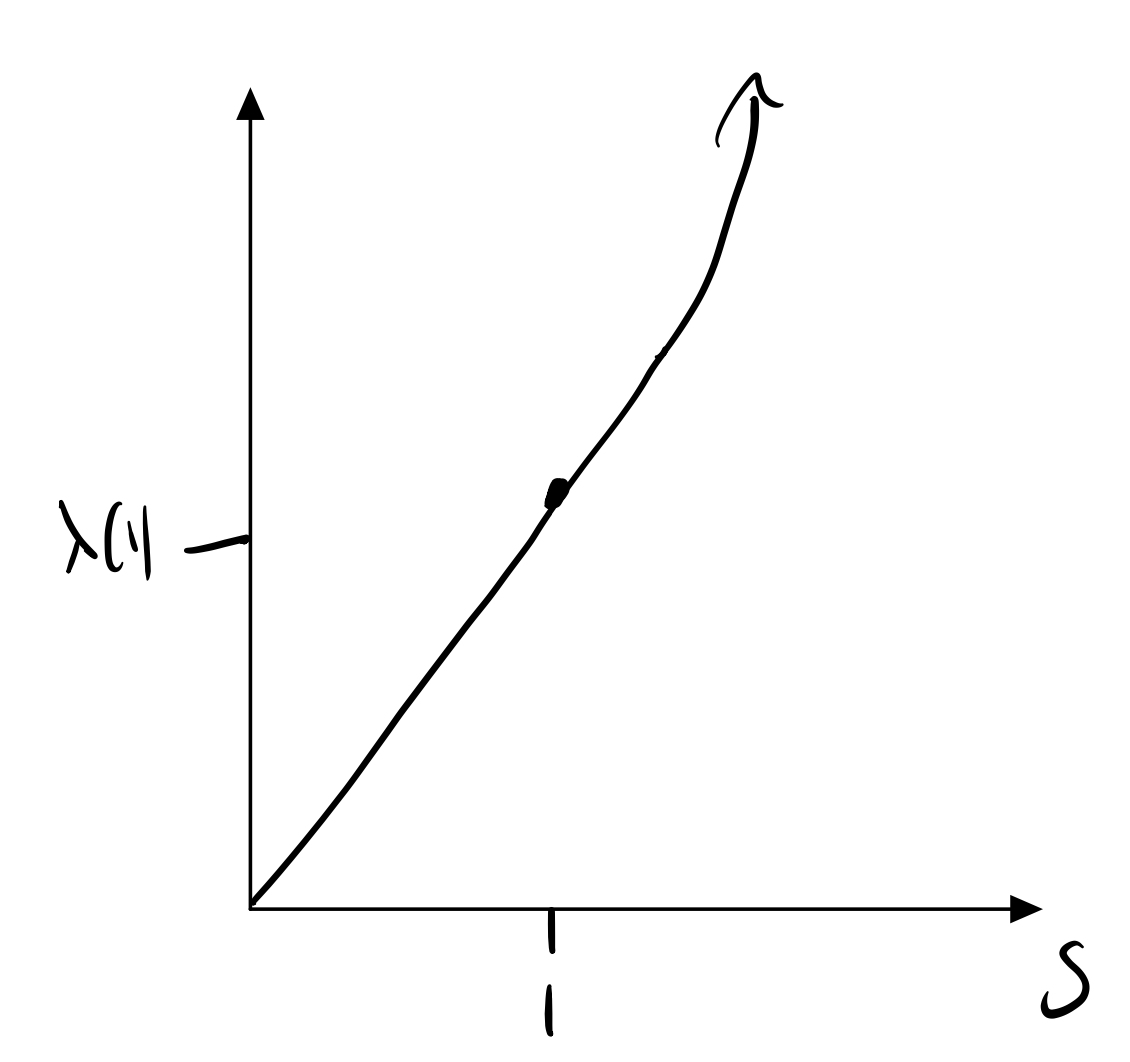
\includegraphics[scale=0.4]{Images/fig-lec30p1.png}
\end{center}

There is a bit of a dimensional transmutation going on here. If we put $m = 0$, then there is no dimensionful parameters in the field theory, but then one has appeared, and we do not know what it is, because the only information we have is our original theory with no dimensionality at all. So, we need to do experiments to figure it out. When TRIUMF says that the QCD is 200MeV is some statement about the... (couldn't follow)

There is a disaster here to note, where there is a crossover from the denominator being positive to negative. This is the Landau pole, and beyond this momentum the theory isn't sensible.

There is in an analysis in the notes of what happens depending on what the beta function looks like. As $s$ diverges, $\beta(\lambda)$ has to be such that $\int_{\lambda_0}^\lambda \frac{d\lambda'}{\beta(\lambda')}$ diverges, which gives us a maximal value of $s$ (couldn't follow). Note this is not fully resolved, and there is the possibility for a maximal scale, or that one does not exist depending on the dependency of $\beta$ on $\lambda$. If there is a maximum scale then this theory is incomplete.

\begin{center}
    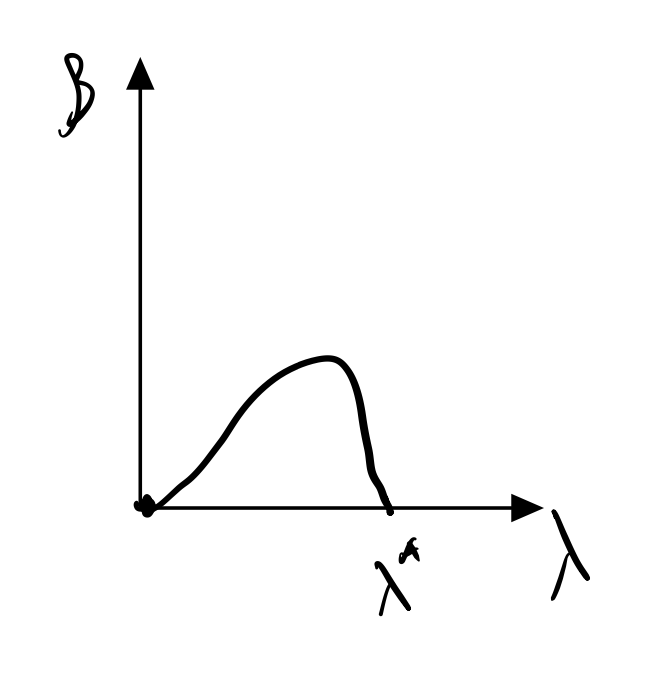
\includegraphics[scale=0.4]{Images/fig-lec30p2.png}
\end{center}

Other possibilities - $\beta$ could have a zero at some fixed point $\lambda = \lambda^*$. If the dimension is 4 this cannot occur, if the dimension is less than 4 then the $\beta$ function has an interesting shape:
\begin{equation}
    \beta(\lambda) = \lambda(2\omega - 4) + \frac{3\lambda^2}{16\pi^2}
\end{equation}
this is the $\beta$ function in a double expansion, one of the parameters being $\lambda$ and the other $2\omega - 4$ (and keeping terms to leading order). This $\beta$ function looks as follows:

Note at high energies we have a flow to zero. This is because the coupling constant has a dimension, so the ratio of the coupling constant to the energy scale is dimensionless, so as the energy scale gets very big, the dimensionless scale gets small (Flows to field theory). On the opposite side, it flows to strong coupling at small momenta, but the nonlinearities in the theory conspire to stop the flow.

\begin{center}
    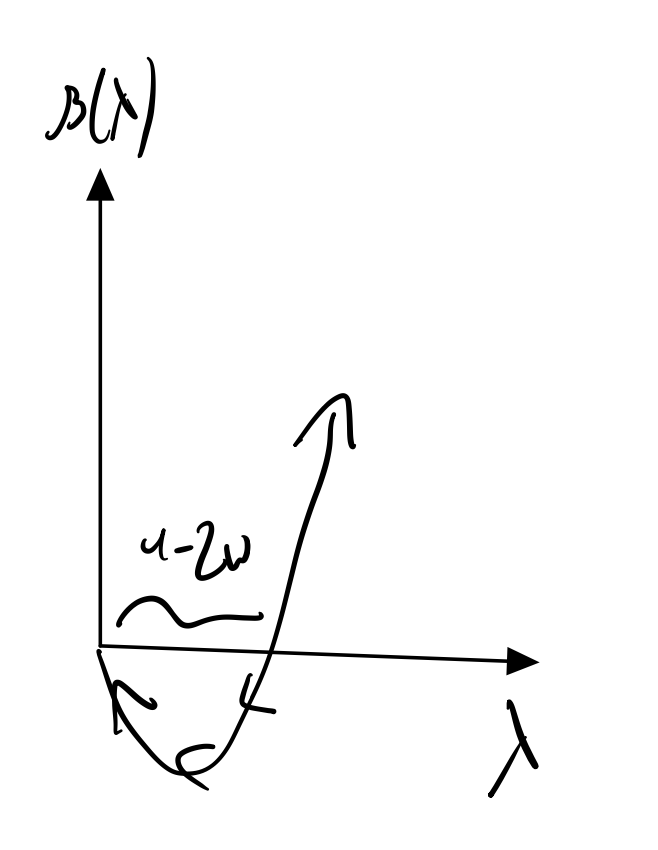
\includegraphics[scale=0.4]{Images/fig-lec30p3.png}
\end{center}

In dimensions less than 4, the theory gets stuck in one regime, and we are therefore able to obtain the entire theory in perturbation theory. $\e$-expansion for the Ising model in $2\omega$ dimensions is very successful because the fixed point is extremely isolated - known as the Wilson-Fisher fixed point.

So, that's the renormalization group - there is a lot more to say but we leave that to a future course.

\subsection{Scattering and the S-Matrix}
So far we have studied the calculation of correlation functions. At some point we have to ask what they are good for. So, let's discuss that. Of course, the condensed matter theorists know that the two-point functions are useful for linear response theory (conductivity of metals etc.) Higher point correlation functions are less useful in CM. But anyway, what about in relativistic field theory? The main thing the correlation functions are useful in this context are in scattering theory.

So let's think about a scattering matrix. What do we do? We make a beam of particles (more or less free particles - far enough apart to not interact). So the energies are just the sum of the energies, the momenta the sum of the momenta etc. We can then model them as free particles. 

In principle the scattering of two particles could create more, but let us work in the low-energy elastic scattering regime. Diagramatically, this may look as follows:

\begin{center}
    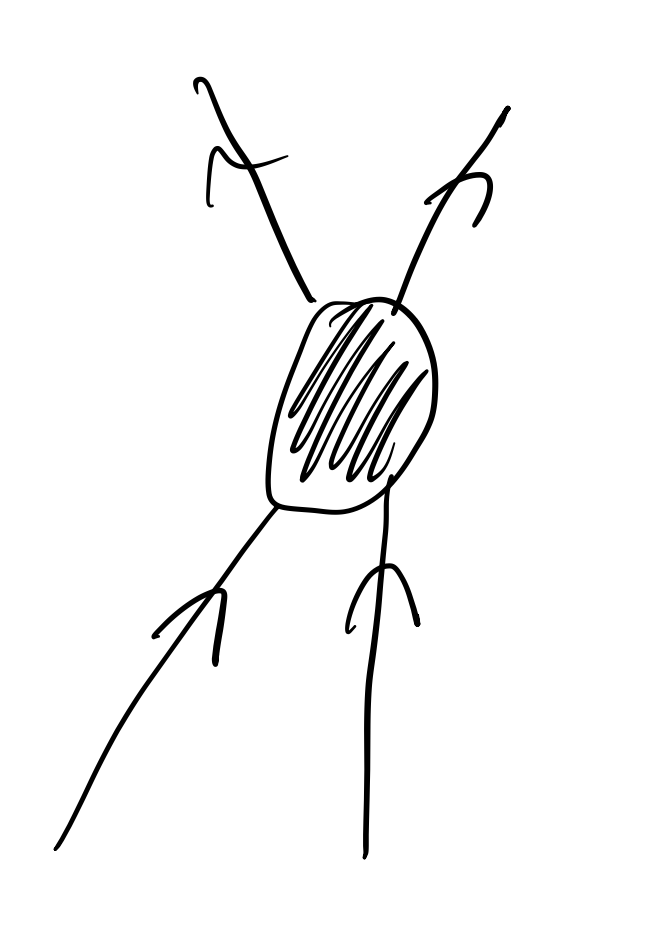
\includegraphics[scale=0.4]{Images/fig-lec30p4.png}
\end{center}

When we detect the particles, they would be far from the other particles, and only interacting with the detectors.

If the initial state of the particles is free incoming particles, we can model them with free fields:
\begin{equation}
    (-\p^2 + m^2)\varphi_{in}(x) = 0
\end{equation}
then something happens which is certainly not free field theory, and we get an outgoing state. We give them enough time to interact, fly out etc. And then we get:
\begin{equation}
    (-\p^2 + m^2)\varphi_{out}(x) = 0
\end{equation}
They might look a bit different than the incoming particles (of course), but they are the same kinds of particles by assumption (e.g. same mass). Of course $\varphi_{in}$ could be an operator which we know everything about (we have studied free field theory to death)... $\varphi_{out}$ is free, but also a bit more subtly as there is now an overlap of wavepackets.

So, we have an incoming state:
\begin{equation}
    \frac{1}{\sqrt{2!}}a^\dag_{in}(\v{k}_1)a_{in}^\dag(\v{k}_2)\ket{0}
\end{equation}
how do we describe the stuff that happened to the free particles? They come out, they are free particles again, so vectors in the same hilbert space, but it should be a mixture of what the incoming states could have been:
\begin{equation}
    \ket{\text{out}} = \sum \ket{\text{in}}S
\end{equation}
where $S$ are the coefficients - the amplitude of finding the free particle states in the final state. This is the \emph{S-matrix}. I can take it to be some operator acting on the incoming state, so let us write the above as:
\begin{equation}
    \ket{\text{out}} = S^\dag \ket{\text{in}}
\end{equation}

There is a beautiful formula for this:
\begin{equation}
    S = \left. :e^{\int d^4x \varphi_{in}(x)(-\p^2 + m^2)\frac{\delta}{\delta J(x)}}:Z[J]\right|_{J = 0}
\end{equation}
where $:$ denotes normal ordering. The fact that $S$ is an operator comes from the fact that $\varphi_{in}$ is an operator on the Fock space. Normal ordering means we put all the $a$s to the right and the $a^\dag$s to the left.

There is a derivation of this that is not very complicated but a bit long. See textbook. To use the formula, one requires the on-shell subtraction scheme. This means that the two-point function should have a pole and residue as if it were a free-field two point function:
\begin{equation}
    D(k^2) = \frac{-i}{k^2 + m^2 - i} + \text{finite as $k^2 \to -m^2$}
\end{equation}
If the counterterms are not chosen in this way, the $m$ would/wouldn't be the actual mass (couldn't follow).

What this does for us is $\frac{\delta}{\delta J}$ inserts a $\varphi$ into the expectation value... we take an $n$-point function generated by the $\frac{\delta}{\delta J}$s... we project:
\begin{equation}
    \int d^4x \frac{e^{ikx}}{\sqrt{(2\pi)^3 2\sqrt{k^2 + m^2}}}(-\p^2 + m^2)\bra{0}T\varphi(x_1) \ldots \varphi(x_n)\ket{0}
\end{equation}
I didn't follow anything that was said about what this represents. But for some reason, we need the $n$-point functions with the external legs amputated. This is not particularly irreducible or connected, it just has an amputation some way or another. For the $\phi^4$ theory this is irreducible.

Next day we'll go through QED, and redo some perturbative things with small additional things that happen in the more complex QED setting.